\documentclass[border=10pt,convert]{standalone}
\usepackage{tikz}
\usepackage[sfdefault,book]{FiraSans}
\usepackage[default]{sourcecodepro}
%\usetikzlibrary{patterns,decorations.pathreplacing,positioning,calc,shapes,chains,backgrounds}
\usetikzlibrary{arrows.meta,calc}
\tikzset{%
  >={Latex[width=2mm,length=2mm]},
  % Specifications for style of nodes:
            base/.style = {rectangle, rounded corners, draw=black,
                           minimum width=3cm, minimum height=2cm,
                           text centered, font=\sffamily\bfseries},
            tool/.style = {font=\ttfamily, draw=black, fill=green!30},
        external/.style = {base, fill=gray!50, font=\sffamily\itshape},
        internal/.style = {base, fill=green!30},
          shards/.style = {font=\ttfamily, draw=black, fill=red!30},
}
\begin{document}    
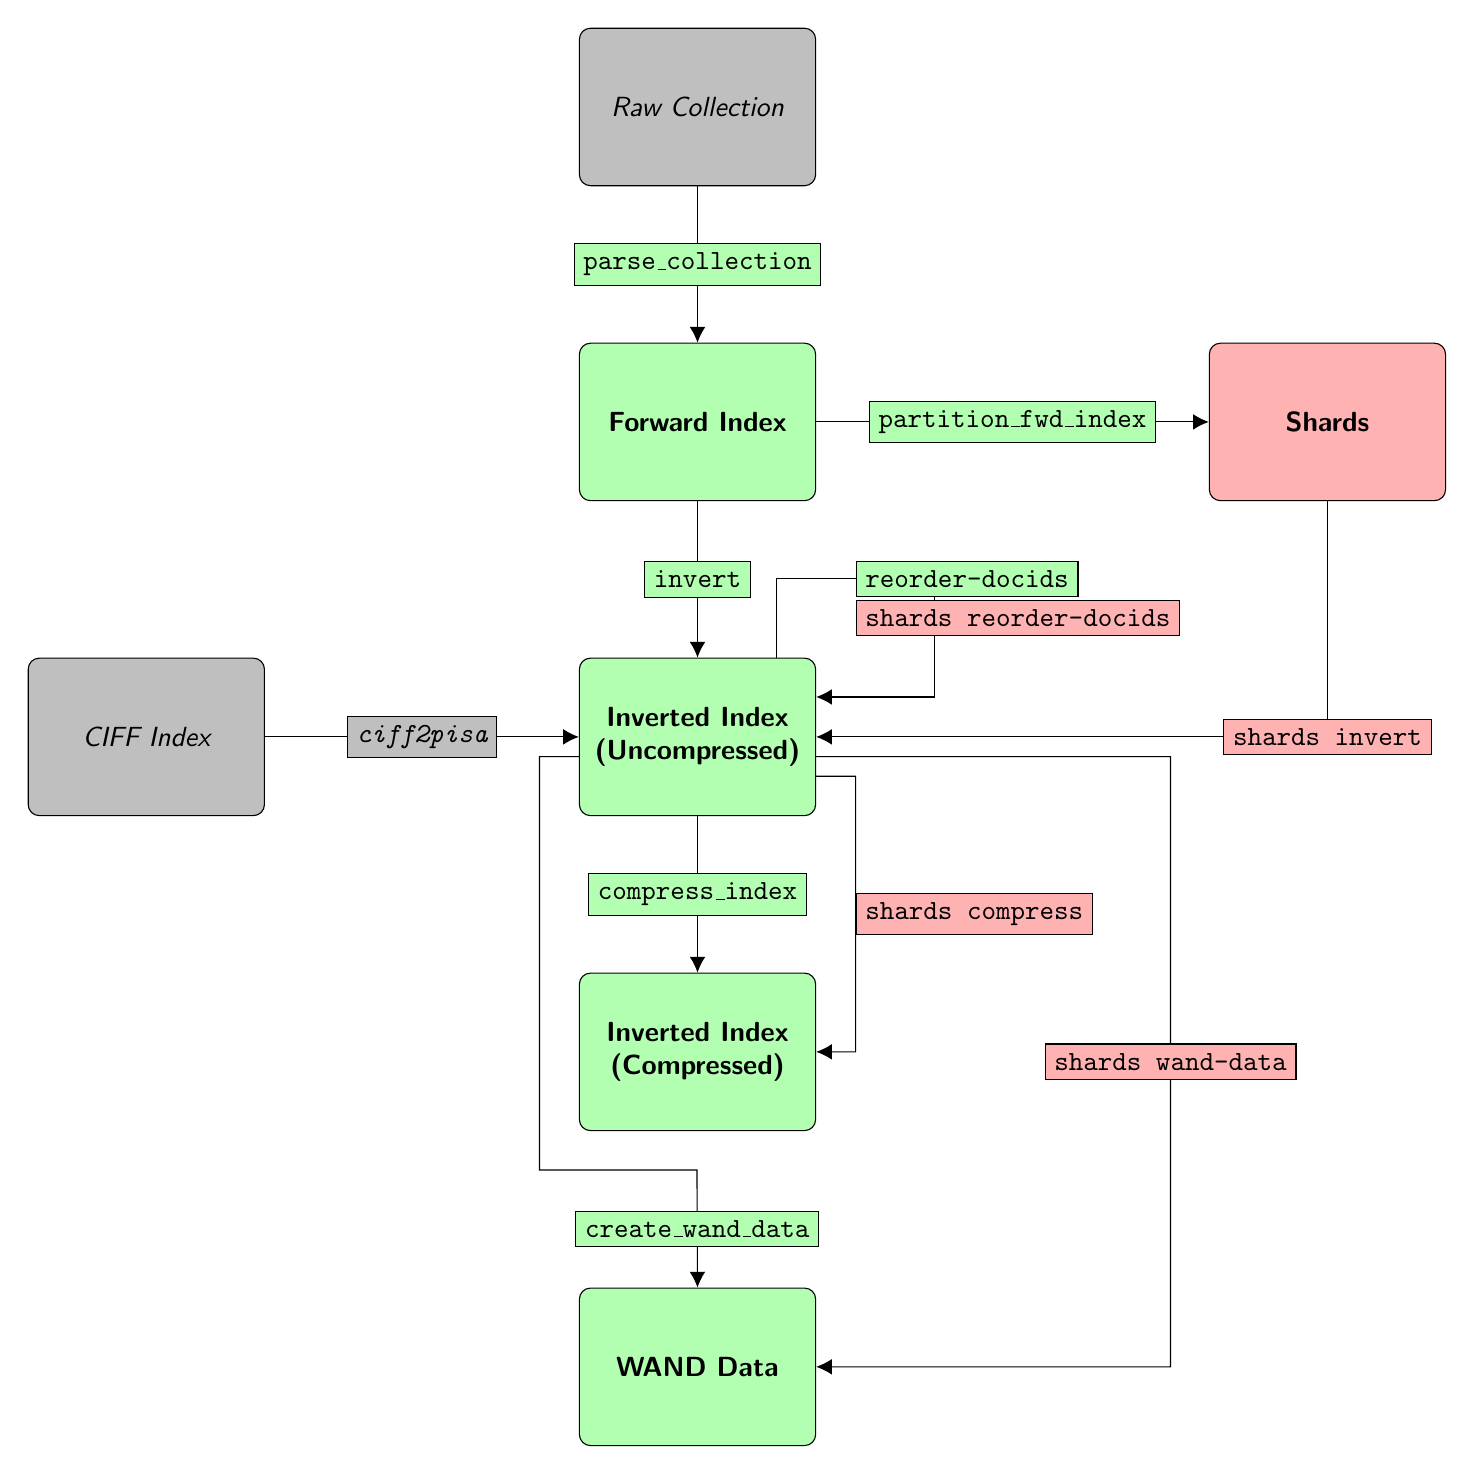
\begin{tikzpicture}[node distance=4cm,
    every node/.style={fill=white, font=\sffamily}, align=center]

  \node (collection)             [external]              {Raw Collection};
  \node (fwd)                    [internal, below of=collection]          {Forward Index};
  \node (inv)                    [internal, below of=fwd]   {Inverted Index\\ (Uncompressed)};
  \node (inv-compressed)         [internal, below of=inv]   {Inverted Index\\ (Compressed)};
  \node (wand)                   [internal, below of=inv-compressed]   {WAND Data};

  \node (ciff)             [external, left of=inv, xshift=-3cm]              {CIFF Index};
  \node (shards)             [base, fill=red!30, right of=fwd, xshift=4cm]              {Shards};

  \draw[->] (collection) -- node [tool] {parse\_collection}     (fwd);
  \draw[->] (fwd)        -- node [tool] {invert}                (inv);
  \draw[->] (inv)        -- node [tool] {compress\_index}       (inv-compressed);
  \draw[->] (ciff)       -- node [tool, fill=gray!50, font=\itshape\ttfamily] {ciff2pisa}             (inv);
  \draw[->] (fwd)        -- node [tool] {partition\_fwd\_index} (shards);
  \draw[->] (shards)     |- node [shards] {shards invert}         (inv);

  \draw[->] ($ (inv.west) + (0, -0.25) $)
      -- ++(-0.5,0)
      -- ++(0,-5.25)
      -- ++(2,0)
      -- node [tool] {create\_wand\_data} (wand.north);

  \draw[->] ($ (inv.east) + (0, -0.5) $)
      -- ++(0.5,0)
      -- node [shards, anchor=west] {shards compress} ++(0,-3.5)
      -- (inv-compressed.east);

  \draw[->] ($ (inv.east) + (0, -0.25) $)
      -- ++(4.5,0)
      -- node [shards] {shards wand-data} ++(0,-7.75)
      -- (wand.east);

  \draw[->] ($ (inv.north east) + (-0.5, 0) $)
      -- ++(0.0,1)
      -- node [name=reorder, tool, anchor=west] {reorder-docids} 
         node [shards, anchor=west, yshift=-0.5cm] {shards reorder-docids} ++(2,0.0)
      -- ++(0.0,-1.5)
      -- ($ (inv.north east) + (0, -0.5) $);

  \end{tikzpicture}
\end{document}
